\subsection{Din\'amica de Fluidos Computacional} \label{DFC}

\noindent
\justify

La \textit{Din\'amica de Fluidos Computacional} (CFD, por sus siglas en ingl\'es) es una herramienta computacional ampliamente usada en ingenier\'ia para el desarrollo de simulaciones num\'ericas que involucren fluidos. Emplea como m\'etodo base el m\'etodo de vol\'umenes finitos (FVM). Este m\'etodo num\'erico transforma las ecuaciones diferenciales parciales, que representan las leyes conservativas, en ecuaciones algebraicas discretas sobre vol\'umenes finitos. 

\noindent
\justify

Inicia con la discretizaci\'on del dominio en elementos no superpuestos. Las ecuaciones diferenciales son discretizadas (transformadas) en ecuaciones algebraicas al integrarlas sobre cada dominio de los elementos. El sistema de ecuaciones algebraicas es luego resulto para calcular los valores de las variables dependientes de cada elemento. Algunos de los t\'etminos en la ecuaci\'on de conservaci\'on se convierten en flujos que se eval\'uan sobre las caras de los elementos. Es `sencillo' evaluar condiciones de frontera, tanto de tipo \textit{Dirichlet} como \textit{Neumann}, de manera no invasiva, dado que las variables desconocidas se eval\'uan en los centroides de los elementos, no en las caras de los mismos, como se aprecia en la Figura \ref{elemento}. Estas caracter\'istias lo hacen adecuado para que la simulaci\'on presente una variedad de aplicaciones que involucran: flujo de fluidos y transferencia de calor y masa.

\noindent
\justify

B\'asicamente, con este m\'etodo num\'erico se busca resolver los siguientes grupos de ecuaciones:

\begin{itemize}
	\item Ecuaci\'on de continuidad:
	\begin{equation*}
		\frac{\partial u}{\partial x} + \frac{\partial v}{\partial y} = 0
	\end{equation*}
	\item Ecuaciones de momento:
	\begin{equation*}
			\frac{\partial u}{\partial t} + u \frac{\partial u}{\partial x} + v \frac{\partial u}{\partial y} = - \frac{1}{\rho} \frac{\partial p}{\partial x} + \frac{\mu}{\rho} \left( \frac{\partial ^2 u}{\partial x ^2} + \frac{\partial ^2 u}{\partial y ^2} \right)
	\end{equation*}
	\begin{equation*}
			\frac{\partial v}{\partial t} + u \frac{\partial v}{\partial x} + v \frac{\partial v}{\partial y} = - \frac{1}{\rho} \frac{\partial p}{\partial y} + \frac{\mu}{\rho} \left( \frac{\partial ^2 v}{\partial x ^2} + \frac{\partial ^2 v}{\partial y ^2} \right)
	\end{equation*}
\end{itemize}

\noindent
\justify

De estas ecuaciones, los componentes desconocidos suelen ser la presi\'on y velocidad. Se requieren condiciones iniciales y de frontera para definir el problema.No hay una ecuaci\'on espec\'ifica para definir la presi\'on. Para flujos incompresibles, la presi\'on es el campo que hace que la velocidad logre cumplir la ley de la conservaci\'on de la masa$^{\cite{Abou-Hweij2020}}$.

\noindent
\justify

Los m\'etodos num\'ericos se enfocan tanto en el proceso de discretizaci\'on como en el m\'etodo de soluci\'on del grupo de ecuaciones algebraicas obtenidas. La \textbf{precisi\'on} de una soluci\'on num\'erica est\'a arraigada al m\'etodo de discretizaci\'on$^{\cite{Bao2021}}$.

\begin{figure}[h!]
	\centering
	\begin{tikzpicture}
 		\draw (0,0) rectangle (12,7);
 		\foreach \x in {1,...,4}{
			\draw (\x*3,0) -- (\x*3,7); 		
 		}
 		\foreach \y in {1,...,3}{
			\draw (0, \y*2.33) -- (12,\y*2.33); 		
 		}	
 		\draw[pattern=north west lines, pattern color=blue!55!red] (3,2.33) rectangle (6,4.66);	
 		\draw[fill=cyan] (4.5,3.5) circle (0.2cm);
 		\draw[-triangle 90, fill=black] (7.5,3.5) -- (4.7,3.5);
 		\node[align=right] at (7.5,3.5) {Centroide del \\ elemento};
 		\node[color=black] at (4.5,3) {Elemento};
 		\draw (9,4.66) circle (0.1cm);
 		\draw[-triangle 90, fill=black] (10.5,5.3) -- (9.15,4.8);
 		\node[align=right] at (10.5,5.5) {(V\'ertice)};
	\end{tikzpicture}
	\caption{Discretizaci\'on del dominio (malla cartesiana).}
	\label{elemento}
\end{figure}

\newpage

\noindent
\justify

Existen dos tipos de mallas para el an\'alisis mediante CFD, como se aprecia en la Figura \ref{mallas}.

\begin{figure}[h!]
	\centering
	\begin{subfigure}[b]{0.48\textwidth}
		\centering
		\begin{adjustbox}{max width = \textwidth}
		\begin{tikzpicture}
			\begin{axis}[grid=both,view={70}{40},colormap/viridis]
  				\addplot3+[surf,mesh/rows=11,mesh/ordering=colwise,no marks] file {malla.txt};
			\end{axis}
		\end{tikzpicture}
		\end{adjustbox}
		\caption{Malla estructurada.}
	\end{subfigure}
	\hfill
	\begin{subfigure}[b]{0.5\textwidth}
		\centering
		\begin{adjustbox}{max width = \textwidth}
		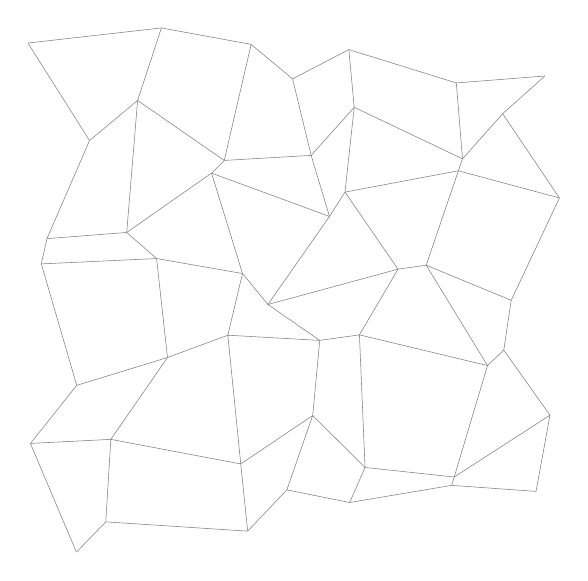
\begin{tikzpicture}
			\foreach \i [evaluate={\ii=int(\i-1);}] in {0,...,6}{
  			\foreach \j [evaluate={\jj=int(\j-1);}] in {0,...,6}{
    			\coordinate [shift={(\j,\i)}] (n-\i-\j) at (rand*190:1/3+rnd/8);
				\ifnum\i>0
  					\draw [help lines] (n-\i-\j) -- (n-\ii-\j);
				\fi
				\ifnum\j>0
  					\draw [help lines] (n-\i-\j) -- (n-\i-\jj);
				\fi
			}}
		\end{tikzpicture}
		\end{adjustbox}
	\caption{Malla no estructurada.}
	\end{subfigure}
	\caption{Tipos de mallas$^{\cite{Roda-Casanova2021}}$.}
	\label{mallas}
\end{figure}

\noindent
\justify

La conversi\'on de las ecuaciones diferenciales parciales requieren la discretizaci\'on del dominio de estudio; que, a su vez, depende de la dimensionalidad del problema.

\subsubsection{Solucionadores}

\noindent
\justify

Existen diferentes m\'etodos de soluci\'on de sistemas de ecuaciones algebraicas que pueden ser: \textit{exactos} o \textit{iterativos}. Los solucionadores que emplean m\'etodos exactos no suelen usarse en simulaciones num\'ericas debido al alto costo computacional. B\'asicamente tratan de resolver el sistema matricial $A \phi = B \rightarrow \phi = A^{-1} B$. 

\noindent
\justify

Los m\'etodos iterativos suelen basarse en la l\'ogica de \textit{suposici\'on} y \textit{corroboraci\'on}. El m\'etodo de Gauss - Seidel$^{\cite{Bai2021}}$, por ejemplo, inicia suponiendo el valor de una variable, corrobor\'andola con el c\'alculo de las dem\'as; en caso de no coincidir, su supone el resultado final de la variable supuesta, donde se vuelve a corroborar hasta que el supuesto y la corroboraci\'on coincidan o hasta que el margen de error sea tolerable.

\subsubsection{Metodolog\'ias de verificaci\'on y validaci\'on} \label{verified}

\noindent
\justify

Tienen por objetivo garantizar el menor \textit{error computacional} posible. Entre ellas se destacan:

\begin{itemize}
	\item \textit{Simple}: estudio de la evoluci\'on global o local de una variable debido al refinamiento de malla, como se aprecia en la Figura \ref{valsimple}.
	\begin{figure}[h!]
	\centering
	\begin{tikzpicture}
		\begin{axis}[
			domain = 0:1000,
			grid = both, minor tick num=2,
			title = \textbf{Validaci\'on por refinamiento de malla},
			xlabel = N\'umero de nodos,
			ylabel = Valor,
			legend pos = outer north east,
			restrict y to domain* = 0:100,
			width=10cm, height=8cm
		]
		\addplot[blue, line width=2pt] {\val};
		\addplot[
        scatter,scatter src=explicit symbolic,
        scatter/classes={
            a={mark=o,black},
            b={mark=triangle*,red},
            c={mark=o,draw=black,fill=black}
        }
    ]
    table[x=x,y=y,meta=label]{
        x	y	label
		10	30	a
		15	32	a
		30	43	a
		60	55	a
		100	70	a
		300	80	a
		600	92	a
		800	95	a
		1000	96	a

    };
		\legend{Te\'orico, Num\'erico};
		\end{axis}
	\end{tikzpicture}
	\caption{M\'etodo de validaci\'on simple.}
	\label{valsimple}
	\end{figure}
	\item \textit{Detallada}: se basa en la extrapolaci\'on generalizada de Richardson y en el \'indice de convergencia de malla (GCI).
	\item \textit{Experimentaci\'on}: se validan los resultados con estudios experimentales.
\end{itemize}

\subsubsection{An\'alisis bidimensional - 2D} \label{CFD2D}

\noindent
\justify

Para an\'alisis bidimensional, se busca resolver la Ecuaci\'on \ref{2DCFD}.

\begin{equation}
\underbrace{\rho \frac{\partial \phi}{\partial t}}_{\text{transitorio}} + \underbrace{\rho u \frac{\partial \phi}{\partial x} + \rho v \frac{\partial \phi}{\partial y}}_{\text{convectivo}} = \underbrace{ \frac{\partial}{\partial x} \left( \Gamma \frac{\partial \phi}{\partial x} \right) + \frac{\partial}{\partial y} \left( \Gamma \frac{\partial \phi}{\partial y} \right)}_{\text{difusivo}} + \underbrace{S_{\phi}}_{\text{fuente}}
\label{2DCFD}
\end{equation}

\noindent
\justify

La discretizaci\'on del dominio se realiza acorde a la Figura \ref{dis2D}.

\begin{figure}[h!]
\centering
\begin{tikzpicture}
\draw (0,0) rectangle (6,6);
\newcounter{contx} %counter
\setcounter{contx}{0}
\newcounter{conty} %counter
\setcounter{conty}{0}
\foreach \x in {0,1.5,3,4.5}
    \foreach \y in {0,1.5,3,4.5}
      {
        \draw (\x,\y) rectangle (\x + 1.5, \y + 1.5);
        \draw[fill=black] (\x + 0.75, \y + 0.75) circle (0.5mm);
        \stepcounter{conty}
        \ifnum \value{contx}<3
        	\draw[red, -triangle 90, fill=red] (\x+1.3, \y + 0.75) -- (\x+1.7, \y + 0.75);
        \fi
        \ifnum \value{conty}=4
        	\setcounter{conty}{0}
        	\stepcounter{contx}
        \else
        	\draw[blue, -triangle 90, fill=blue] (\x+0.75, \y + 1.3) -- (\x+0.75, \y + 1.7);
        \fi
      }

\foreach \x in {0,1.5,3,4.5}
	{
		\draw[fill=black] (\x + 0.75, 0) circle (0.5mm);
		\draw[fill=black] (\x + 0.75, 6) circle (0.5mm);
	}

\foreach \y in {0,1.5,3,4.5}
	{
		\draw[fill=black] (0, \y + 0.75) circle (0.5mm);
		\draw[fill=black] (6, \y + 0.75) circle (0.5mm);
	}

\node at (2.5,2.5) {P};
\node at (4,2.5) {E};
\node at (2.5,4) {N};
\node at (2.5,1) {S};
\node at (1,2.5) {W};

\end{tikzpicture}
\caption{Discretizaci\'on dominio bidimensional.}
\label{dis2D}
\end{figure}

\noindent
\justify

Existen diferentes enfoques para el an\'alisis de problemas bidimensionales, entre ellos se encuentran: diferencias centradas, \textit{upwind} e h\'ibrido. El acercamiento por diferencias centradas asume una variaci\'on lineal de $\phi$ entre nodos para una malla uniforme, de modo que:

\begin{equation}
\begin{array}{c}
	a_P \phi _P = a_E \phi _E  + a_W \phi _W + a_N \phi _N + a_S \phi _S + b \\
	a_E = D_e - F_e/2 \\
	a_W = D_w + F_w/2 \\
	a_N = D_n - F_n/2 \\
	a_S = D_s + F_s/2 \\
	a_P = a_E + a_W + a_N + a_S + \rho \frac{\Delta x \Delta y}{\Delta t} + \left(F_e - F_w + F_n - F_s \right) \\
	b = \rho \frac{\Delta x \Delta y}{\Delta t} \phi _P ^0 + S \Delta x \Delta y
\end{array}
\end{equation}